%=============================================================================
%=============================================================================

\chapter{Babel-based Interfaces}
\label{ch-babel}

\section{Introduction}

Much of \hypre{} is accessible through a multi-language interface
built through the Babel tool.  This tool can connect to \hypre{} from
your code which you can write in any of several languages.

The Struct (Structured grid), SStruct (Semi-Structured grid), and IJ
(linear algebra style) interfaces all can be used
this way.  The code you write to call \hypre{} functions through the
Babel-based interface works much the same as the code you write to
call them through the original C interface.  The function names are
different, the object structure of \hypre{} is more visible, and there
are many more minor differences.

This chapter will discuss these differences and present brief
examples.  You can also see them in action by looking at the complete
examples in the examples directory.

You do not need to have the Babel software to use the Babel-based
interface of \hypre{}.  Prebuilt interfaces for the C, C++, and
Fortran languages are included with the \hypre{} distribution.  We
will enlarge the distribution with more such interfaces whenever \hypre{}
users indicate that they need them, and our tools such as Babel
support them.  Although you do not need to know about Babel to use the
Babel-based interface of \hypre{}, if you are curious about Babel you
can look at its documentation at \url{http://www.llnl.gov/CASC/components}.

% >>> Someplace we should say that we can't do Python until shared
% >>> library support is put back into hypre (it would be better to be
% >>> able to build shared libraries again!)

\section{The HYPRE Object Structure}

Even though it is written in C, \hypre{} is object-oriented in its
conceptual design.  The object structure of \hypre{} is often visible
in names of structs and functions.  Because Babel is explicitly
object-oriented, the Babel-based interface of \hypre{} makes the
\hypre{} object system more visible, at least at the level of the
user interface.  Understanding the \hypre{} object structure can be
helpful but is not necessary for using \hypre{} and its Babel
interface.

The object structure of the Babel-based interface is explicitly
defined in the SIDL (Scientific Interface Definition Language) file
\code{Interfaces.idl}.  Babel translates this object structure as
appropriate for the language the user uses - from SIDL's interfaces
and classes to C++ classes, or to mangled names in C and Fortran.
For more information about the SIDL language, visit the Babel project
website, \url{http://www.llnl.gov/CASC/components}.

Here is an example: In the SIDL file defining the Babel interface, the
StructVector class inherits from the StructVectorView and Vector
interfaces.  StructVectorView extends MatrixVectorView interface,
which extends the ProblemDefinition interface.  The Babel StructVector
class can appear as a C++ class also named \code{StructVector} (in the
\code{bHYPRE} namespace), as a C struct named
\code{bHYPRE_StructVector}, or as a Fortran
\code{integer*8}.  Its member function SetValues can appear in C++ as a
member function \code{SetValues}, in C as a function
\code{bHYPRE_StructVector_SetValues}, or in Fortran as a subroutine
\code{bHYPRE_StructVector_SetValues}.

The inheritance structure matters in use because you can cast an
object up and down its inheritance hierarchy.  Sometimes you must cast
it in order to provide an object of the right data type in a function
call.  For example, the PCG solver works on any kind of vector, so PCG
functions expect Vector objects among their arguments.  If you have a
StructVector, and you want to use PCG, you might write C and Fortran
code containing cast functions like the following.  In C++, of course,
such explicit casts are unnecessary.
\begin{verbatim}
    bHYPRE_StructVector b_S = bHYPRE_StructVector_Create(...);
    bHYPRE_Vector       b = bHYPRE_Vector__cast( b_S );
    hypre_Vector        x;
    bHYPRE_PCG          PCG_solver;
    bHYPRE_PCG_Apply( PCG_solver, b, &x );
\end{verbatim}
\begin{verbatim}
      integer*8 b_S
      integer*8 b
      integer*8 x
      integer*8 PCG_solver
      call bHYPRE_StructVector_Create_f(...,b_S)
      call bHYPRE_Vector__cast_f( b_S, b )
      call bHYPRE_PCG_Apply_f( PCG_solver, b, x, ierr )
\end{verbatim}
(Other code not shown would set up the matrix, provide it and
parameters to the solver, set up the vectors, and so forth).

Figure~\ref{figObjectModel} describes in abbreviated form the most
important ideas of the \hypre{} inheritance hierarchy.


\begin{figure}
\centering
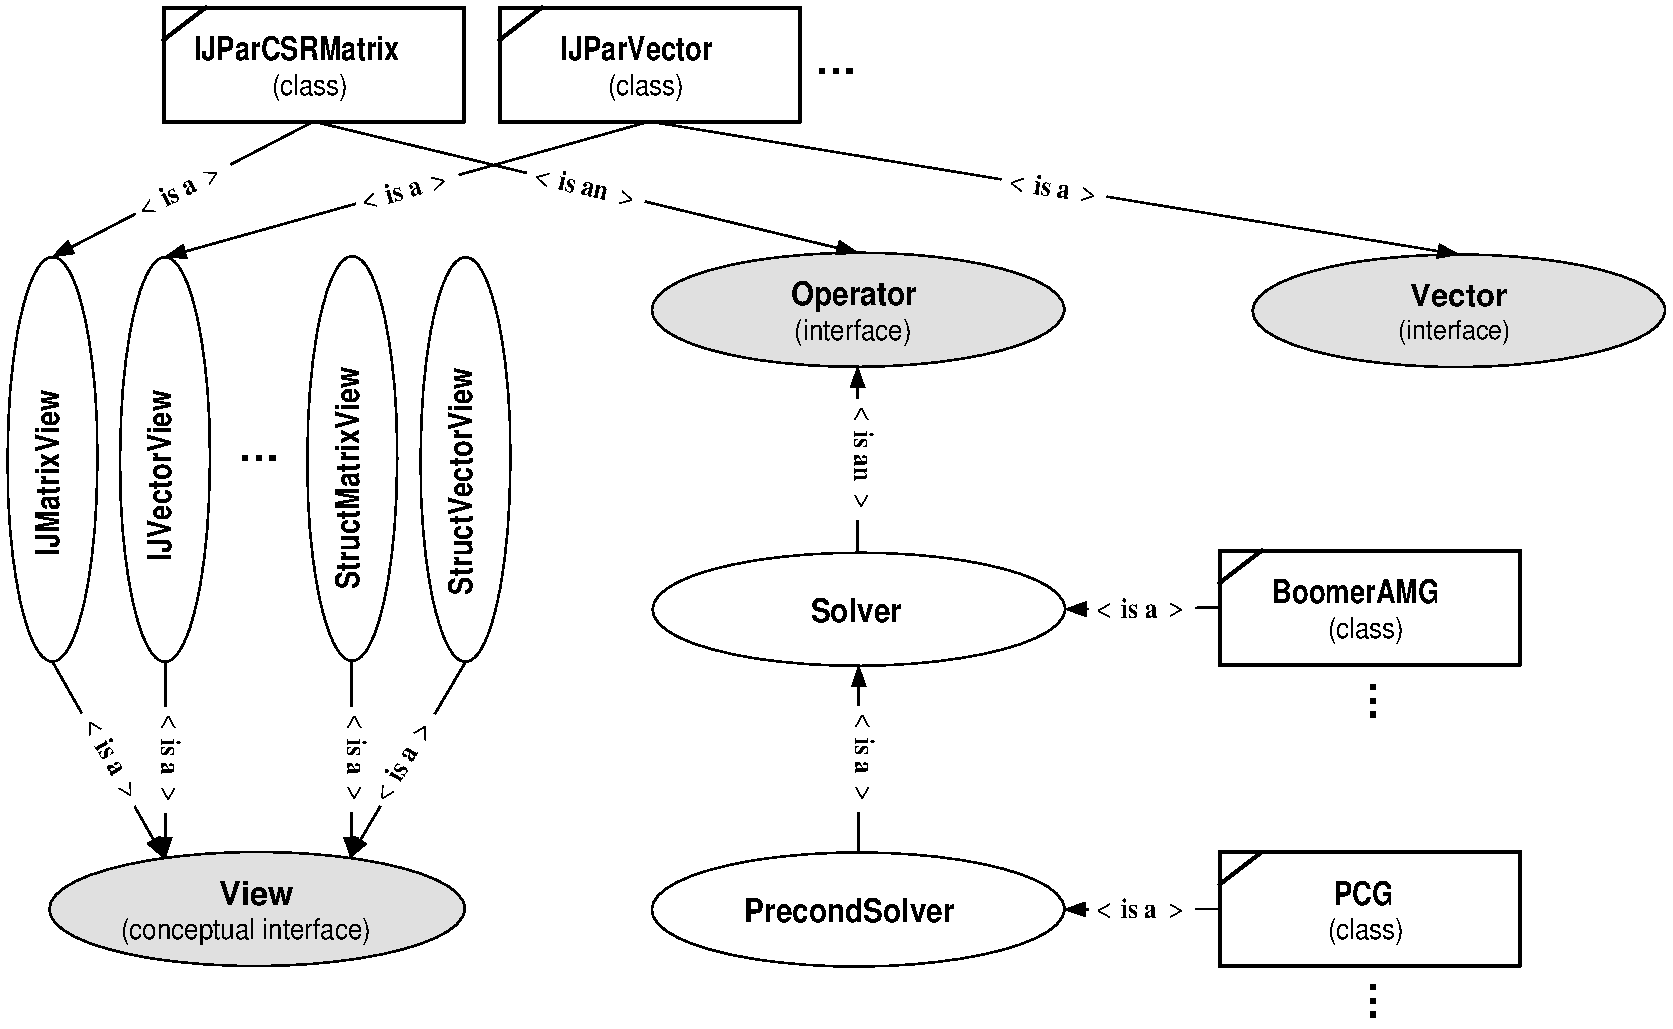
\includegraphics[width=5in]{figObjectModel}
\caption{%
Graphic illustrating the ideas of the object model.}
\label{figObjectModel}
\end{figure}

% The same chart appears in the following two places, among others.
% 1. page 5 of ``The Design and Implementation of hypre, a Library of
% Parallel High Performance Preconditioners''
% (jfp has this in an email from Rob Falgout on May 13, 2005)
% 2. slide 79 of ACTS viewgraphs on hypre dated August 23, 2005 (jfp
% has this in an email from Rob Falgout dated July 19, 2006)


% >>>>>>> a more complete chart would be nice, if it would fit! <<<<<<<<

% >>>>>>> a verbal description of the object system, e.g. what is a
% view, is ESSENTIAL ! <<<<<<<<<
% concepts to include:
% conceptual interface (e.g. IJ) vs 'underlying storage type' (e.g. ParCSR)

\section{Names and Conventions}

In the C-only interface, most \hypre{} function names look like
\code{HYPRE_ClassFunction} where \code{Class} is a class name and
\code{Function} is a (conceptual) function name.  The C-Babel
interface is similar: most function names look like
\code{bHYPRE_Class_Function}.  In the Fortran-Babel interface, most
function names look like \code{bHYPRE_Class_Function_f}.  In the
C++-Babel interface, SIDL (Babel) classes are actually implemented as
classes, so functions look like Class.Function.  In C++, the
Babel-interface functions live in the namespace \code{::ucxx::bHYPRE}.

This function naming pattern is slightly broken in the case of service
functions provided by Babel rather than \hypre{}.  All of them contain
a double underscore, \code{__}.  These functions are used for casting,
certain arrays, and sometimes memory management.  For more information
see the sections on object structure, arrays, and memory management.

Most functions are member functions of a class.  In
non-object-oriented languages, the first argument of the function will
be the object which ``owns'' the function.  For example, to solve
equations with a PCG solver you ``apply'' it to vectors using its
member function \code{Apply}.  In C++, C, and Fortran this concept is
expressed as:
\begin{verbatim}
      pcg_solver.Apply( b, x );   (C++;in the ::ucxx::bHYPRE namespace)
      bHYPRE_PCG_Apply( PCG_solver, b, &x );   (C)
      call bHYPRE_PCG_Apply_f( PCG_solver, b, x, ierr )   (Fortran)
\end{verbatim}

In the Babel interface, data types usually look like \code{Class} in
C, \code{bHYPRE_Class} in C, and \code{integer*8} in Fortran.  Similar
data types in the C-only interface would look like
\code{HYPRE_Class}.  Here \code{Class} is a class name where the
interface is defined in the SIDL file \code{Interfaces.idl}.
Sometimes the class name is slightly different in the C-only
interface, but usually they are the same.

Most \hypre{} objects need to be supplied with an MPI communicator.
The Babel interface has a special class for the MPI communicator; for
details see the section on MPI communicators.

\section{Arrays}
Babel supports a two different kinds of array.  In the \hypre{}
Babel-based interface, almost all the arrays are ``raw arrays'' or
``rarrays'', the native array of the language you use.  And all our
rarrays are one-dimensional arrays.  Thus, you will almost always deal
with arrays as in the following examples of an array \code{rows} for
C, C++, and Fortran.

\begin{verbatim}
      /* C */
      int    *rows;
      rows = calloc( size, sizeof(int) );
      for ( i=0; i<size; i++ )
         rows[i] = ilower + i;
      bHYPRE_IJParCSRVector_SetValues( b, size, rows, values );
      free(rows);

      // C++
      int    *rows;
      rows = new int[size];
      for ( i=0; i<size; i++ )
         rows[i] = ilower + i;
      b.SetValues( size, rows, values );
      delete[] rows;

c     Fortran
      integer    rows(MAX_SIZE)
      do i = 1, local_size
         rows(i) = ilower + i -1
      enddo
      call bHYPRE_IJParCSRVector_SetValues_f(
     1     par_b, size, rows, values, ierr )
\end{verbatim}

The other kind of Babel array is the ``SIDL array'', which has more
structure than the arrays native to languages like C or Fortran - it
accomodates reference counting and knows its own size, for example.
In the \hypre{} Babel-based interface, we presently use SIDL arrays
only for output-only arrays in two functions, GetRow and
CoefficientAccess. In the past they have been used for two-dimensional
input arrays as well.

The following examples show a way to declare, read, and destroy a SIDL
array (see the section on Memory Management for more about the
deleteRef function).  The GetRow and CoefficentAccess functions create
their output arrays, so there is no need to create your own.  For more
information, read the Babel documentation at
\url{http://www.llnl.gov/CASC/components}.

% I've never done any of this.  This should be put in the test
% programs sometime.

\subsubsection{C}
\begin{verbatim}
    struct sidl_int__array *row_js;
    struct sidl_double__array *row_data;
    bHYPRE_IJParCSRMatrix_GetRow( A, i, &row_size, &row_js, &row_data );
    for ( k=0; k<row_size; ++k )
       col[k]  = sidl_int__array_get1( row_js, k );
       data[k] = sidl_double__array_get1( row_data, k );
   sidl_int__array_deleteRef( row_j );
   sidl_double__array_deleteRef( row_data );
\end{verbatim}
\subsubsection{Fortran}
\begin{verbatim}
      integer*8 row_js;
      integer*8 row_data;
      call bHYPRE_IJParCSRMatrix_GetRow_f( A, i, row_size, row_js, row_data )
      do k = 1, row_size
         call sidl_int__array_get1_f( row_js, k-1, col(k) )
         call sidl_double__array_get1_f( row_data, k-1, data(k) )
      enddo
      call sidl_int__array_deleteRef( row_j )
      call sidl_double__array_deleteRef( row_data )
\end{verbatim}


\section{Memory Management}

Babel references-counts all its objects, ``object'' meaning here an
instance of a SIDL class.  Reference counting means that the object
contains an integer which counts the number of outside references to
the object.  The purpose of reference counting is to make sure that an
object gets automatically deleted at exactly the right time - when it
is no longer needed.

With Babel, reference counting is automatic in C++.  But in other
Babel-supported languages you will need to insert a few function calls
to make memory management work.

When you create an object, you get a pointer and normally assign it to
a variable, say \code{Object}.  At that point the object's reference
count starts as 1.  If you copy the pointer,
e.g. \code{SameObject=Object}, you have two references to the same
object.  So you should make sure that the object's reference count
goes up to 2.  You do that with a call of the Babel \code{addRef}
function, as in the following examples.

If you put a Babel object into a struct, or return one through a
function call, you are making a copy.  You will need to call
\code{addRef} at about the time you do this.

You also need to decrement the reference count if one of your
references to an object disappears.  In the above example, if
\code{SameObject} were declared within the scope of the function
\code{MyFunction}, you would need to decrement the reference count
before \code{MyFunction} returns.  You do that by calling the Babel
\code{deleteRef} function, as in the following examples.  For every
object creation, and every \code{addRef} function call, there should
be a corresponding \code{deleteRef} call.

In the simplest and most typical use, you won't copy pointers, so
there is no need for \code{addRef} calls.  But before the end of your
program, or the end of the function which calls \hypre{} through the
Babel interface, you will need to call \code{deleteRef} for every
Babel object which has been created and returned to you.

When a copy is made and abandoned within a short simple stretch of
code, most people can get away without inserting an \code{addRef},
\code{deleteRef} pair.

Here is an example in C showing the life of a vector (the type
\code{bHYPRE_IJParCSRVector} is actually a pointer).  In C:
\begin{verbatim}
    bHYPRE_IJParCSRVector b;
    b = bHYPRE_IJParCSRVector_Create( mpi_comm, ilower, iupper );
    /* do something with b here */
    bHYPRE_IJParCSRVector_deleteRef( b );
\end{verbatim}

If you copy the object, there's a bit more to do.  This example makes
two copies, one with an assignment operator, and one with a cast.  The
argument of \code{addRef} and \code{deleteRef} doesn't matter as long
as it points to the right object, and the data type is what the
function needs.

\begin{verbatim}
    bHYPRE_IJParCSRVector b, b2;
    bHYPRE_Vector vb;
    b = bHYPRE_IJParCSRVector_Create( mpi_comm, ilower, iupper );
    b2 = b;
    bHYPRE_IJParCSRVector_addRef( b );
    vb = bHYPRE_Vector__cast( b );
    bHYPRE_IJParCSRVector_addRef( b );
    /* do something with b,b2,vb here */
    bHYPRE_IJParCSRVector_deleteRef( b );
    bHYPRE_IJParCSRVector_deleteRef( b );
    bHYPRE_IJParCSRVector_deleteRef( b );
\end{verbatim}

This example is just the same, but with a minimum of reference
counting calls.
\begin{verbatim}
    bHYPRE_IJParCSRVector b, b2;
    bHYPRE_Vector vb;
    b = bHYPRE_IJParCSRVector_Create( mpi_comm, ilower, iupper );
    b2 = b;
    vb = bHYPRE_Vector__cast( b );
    /* do something short and simple with b,b2,vb here */
    bHYPRE_IJParCSRVector_deleteRef( b );
\end{verbatim}



Memory management is easier in C++.  Babel objects are ``smart
pointers'', meaning that \code{addRef} and \code{deleteRef} calls are
handled automatically wherever possible.

Following are the above examples in Fortran.

\begin{verbatim}
      integer*8 b
      call bHYPRE_IJParCSRVector_Create_f( mpi_comm, ilower, iupper, b )
c     do something with b here
      call bHYPRE_IJParCSRVector_deleteRef_f( b )
\end{verbatim}

\begin{verbatim}
      integer*8 b, b2
      integer*8 vb
      call bHYPRE_IJParCSRVector_Create_f( mpi_comm, ilower, iupper, b )
      b2 = b
      call bHYPRE_IJParCSRVector_addRef_f( b )
      call bHYPRE_Vector__cast_f( b, vb )
      call bHYPRE_IJParCSRVector_addRef_f( b )
c     do something with b,b2,vb here
      call bHYPRE_IJParCSRVector_deleteRef_f( b )
      call bHYPRE_IJParCSRVector_deleteRef_f( b )
      call bHYPRE_IJParCSRVector_deleteRef_f( b )
\end{verbatim}

\begin{verbatim}
      integer*8 b, b2
      integer*8 vb
      call bHYPRE_IJParCSRVector_Create_f( mpi_comm, ilower, iupper, b )
      b2 = b
      call bHYPRE_Vector__cast_f( b, vb )
c     do something short and simple with b,b2,vb here
      call bHYPRE_IJParCSRVector_deleteRef_f( b )
\end{verbatim}



\section{Matrices and Vectors}

\subsection{ParCSR Matrices}

\subsubsection{C-Babel}
In C with the Babel-based interface, a ParCSR matrix is typically built as follows:

\begin{verbatim}
    bHYPRE_MPICommunicator mpi_comm;
    bHYPRE_IJParCSRMatrix parcsr_A;
    parcsr_A = bHYPRE_IJParCSRMatrix_Create(
      mpi_comm, row_lower, row_upper, col_lower, col_upper );

    bHYPRE_IJParCSRMatrix_Initialize( parcsr_A );

    /* SetValues sets values for matrix rows; normally there
       are many SetValues calls inside a loop ... */
    bHYPRE_IJParCSRMatrix_SetValues( parcsr_A, n_rows, n_cols, rows, cols, values, n_nonzeros );

    bHYPRE_IJParCSRMatrix_Assemble( parcsr_A );
\end{verbatim}

\subsubsection{C-only}
The same job in the C-only interface would be done as follows:

\begin{verbatim}
    MPI_COMM mpi_comm;
    HYPRE_IJMatrix A;
    HYPRE_IJMatrixCreate( mpi_comm, row_lower, row_upper, col_lower, col_upper, &A );

    HYPRE_IJMatrixSetObjectType( A, HYPRE_PARCSR );

    HYPRE_IJMatrixInitialize( A );

    /* SetValues sets values for matrix rows; normally there
       are many SetValues calls inside a loop ... */
    HYPRE_IJMatrixSetValues( A, n_rows, n_cols, rows, cols, values );

    HYPRE_IJMatrixAssemble(A);
\end{verbatim}


The most significant difference between the C-Babel and C-only
interfaces is that the C-only interface includes a SetObjectType
function call not found in the C-Babel interface.  This is because the
same information is incorporated in function names in the Babel
interface.  It is also notable that the MPI communicator is wrapped in
a special object in the Babel interface, but passed directly in the
C-only interface.  This is because the Babel interface is
language-neutral, but MPI communicator types are generally
language-dependent.  MPI communicators are discussed in another
section of this chapter.

\subsubsection{C++-Babel}
Here is how the same matrix would be built in C++ and Fortran.
both with the same Babel-based interface as above.
You can see how everything works the same.  Most of this chapter
will not include non-C examples except in contexts where their differences
from C are interesting.

\begin{verbatim}
    using namespace ::ucxx::bHYPRE;
    MPICommunicator mpi_comm;
    IJParCSRMatrix parcsr_A;
    parcsr_A = IJParCSRMatrix::Create(
       mpi_comm, row_lower, row_upper, col_lower, colupper );

    parcsr_A.Initialize();

    // SetValues sets values for matrix rows; normally there
    //   are many SetValues calls inside a loop ...
    parcsr_A.SetValues( n_rows, n_cols, rows, cols, values, n_nonzeros );

    parcsr_A.Assemble();
\end{verbatim}


\subsubsection{Fortran-Babel}
\begin{verbatim}
          integer*8  bHYPRE_mpicomm
          integer*8  parcsr_A
          call bHYPRE_IJParCSRMatrix_Create_f( bHYPRE_mpicomm, row_lower,
         1     row_upper, col_lower, col_upper, parcsr_A )

          call bHYPRE_IJParCSRMatrix_Initialize_f( parcsr_A, ierrtmp )

    c        SetValues sets values for matrix rows; normally there
    c        are many SetValues calls inside a loop ...
             call bHYPRE_IJParCSRMatrix_SetValues_f(
         1        parcsr_A, n_rows, n_cols, rows, cols, values,
         2        n_nonzeros, ierrtmp )

          call bHYPRE_IJParCSRMatrix_Assemble_f( parcsr_A, ierrtmp )
\end{verbatim}



\subsection{Struct Matrices}

Struct matrices are built almost the same way with
the C-only and Babel+C interfaces.

\subsubsection{C-Babel}

In C, a Struct  matrix is typically built as follows with
the Babel interface:

\begin{verbatim}
    bHYPRE_MPICommunicator mpi_comm;
    bHYPRE_StructMatrix  A_b;
    bHYPRE_StructGrid grid;
    bHYPRE_StructStencil stencil;
    int *box_lower, *box_upper, *stencil_indices;
    double *values;

    A_b = bHYPRE_StructMatrix_Create( mpi_comm, grid, stencil );
    ierr += bHYPRE_StructMatrix_Initialize( A_b );

    /* SetBox values sets values for a block of the matrix;
       normally there are many SetBoxValues calls inside a loop.*/
    bHYPRE_StructMatrix_SetBoxValues(
                  A_b, box_lower, box_upper, dim,
                  stencil_size, stencil_indices, values, volume );
    ierr += bHYPRE_StructMatrix_Assemble( A_b );
\end{verbatim}


Other languages work the same way in the Babel interface; see the
section on ParCSR matrices for syntax examples.

\subsubsection{C-only}

This job is done as follows with the C-only interface:

\begin{verbatim}
    MPICommunicator mpi_comm;
    HYPRE_StructMatrix  A;
    HYPRE_StructGrid    grid;
    HYPRE_StructStencil stencil;
    int *box_lower, *box_upper, *stencil_indices;
    double *values;

    HYPRE_StructMatrixCreate( mpi_comm, grid, stencil, &A);
    HYPRE_StructMatrixInitialize(A);

    /* SetBox values sets values for a block of the matrix;
       normally there are many SetBoxValues calls inside a loop.*/
    HYPRE_StructMatrixSetBoxValues( A, box_lower, box_upper,
                                    stencil_size, stencil_indices, values);
    HYPRE_StructMatrixAssemble(A);
\end{verbatim}


Both interfaces work the same way, with minor differences in argument
lists and data types.

\subsection{SStruct Matrices}

SStruct matrices are built almost the same way with
the C-only and C-Babel interfaces.

\subsubsection{C-Babel}

In C, a SStruct  matrix is typically built as follows with
the Babel interface.  There are minor differences depending on the
kind of SStruct matrix, \code{object_type} in the following.  Its possible
values are \code{HYPRE_PARCSR}, \code{HYPRE_STRUCT}, \code{HYPRE_SSTRUCT}.

For \code{object_type==HYPRE_PARCSR}:
\begin{verbatim}
    bHYPRE_MPICommunicator mpi_comm;
    bHYPRE_SStructParCSRMatrix   A_b;
    bHYPRE_SStructGraph   graph;
    int object_type, dim, var, nentries, nvalues, part;
    int box_lower[3], box_upper[3], index[3];
    int *entries;

    A_b = bHYPRE_SStructParCSRMatrix_Create( mpi_comm, graph );

    /* No call of SetObjectType is needed, the information is in
       the name of this Initialize function: */
    bHYPRE_SStructParCSRMatrix_Initialize( A_b );

    /* SetBoxValues and SetValues are normally called inside loops */
    bHYPRE_SStructParCSRMatrix_SetBoxValues
          ( A_b, part, box_lower, box_upper, dim, var,
            nentries, entries, values, nvalues );
           }
    bHYPRE_SStructParCSRMatrix_SetValues
          ( A_b, part, index, dim, var, nentries, entries, values );

    bHYPRE_SStructParCSRMatrix_Assemble( A_b );
\end{verbatim}


For \code{object_type==HYPRE_STRUCT} or \code{HYPRE_SSTRUCT}:
\begin{verbatim}
    bHYPRE_MPICommunicator mpi_comm;
    bHYPRE_SStructMatrix  A_b;
    bHYPRE_SStructGraph   graph;
    int object_type, n_dim, var, nentries, nvalues;
    int box_lower[3], box_upper[3], index[3];
    int *entries;

    A_b = bHYPRE_SStructMatrix_Create( mpi_comm, graph );

    bHYPRE_SStructMatrix_SetObjectType(A_b, object_type);
    bHYPRE_SStructMatrix_Initialize( A_b );

    /* SetBoxValues and SetValues are normally called inside loops */
     bHYPRE_SStructMatrix_SetBoxValues
           ( A_b, part, boxlower, box_upper, dim, var,
             nentries, entries, values, nvalues );
     bHYPRE_SStructMatrix_SetValues
           ( A_b, part, index, dim, var, nentries, entries, values );

     bHYPRE_SStructMatrix_Assemble( A_b );
\end{verbatim}

\subsubsection{C-only}

The C-only interface is very similar:
\begin{verbatim}
    MPICommunicator mpi_comm;
    HYPRE_SStructMatrix   A;
    HYPRE_SStructGraph    graph;
    int object_type, var, nentries;
    int box_lower[3], box_upper[3], index[3];
    int *entries;

    HYPRE_SStructMatrixCreate( mpi_comm, graph, &A );

    /* HYPRE_SSTRUCT is the default, so we don't have to call SetObjectType */
    if ( object_type != HYPRE_SSTRUCT )
        HYPRE_SStructMatrixSetObjectType(A, object_type);
    HYPRE_SStructMatrixInitialize(A);

    /* SetBoxValues and SetValues are normally called inside loops */
    HYPRE_SStructMatrixSetBoxValues( A, part, box_lower, box_upper, var,
                                     nentries, entries, values );
    HYPRE_SStructMatrixSetValues
         ( A, part, index, var, nentries, entries, values )

    HYPRE_SStructMatrixAssemble(A);
\end{verbatim}


\section{Parameters and Error Flags}

Most \hypre{} objects can be modified by setting parameters.  In the
C-only interface, there is a separate function to set each parameter.
The Babel-based interface has just a few parameter-setting functions
for each object.  The parameters are identified by their names, as
strings.  See below for some examples.

Most \hypre{} functions return error flags, as discussed elsewhere in
this manual. The following examples simply show how they are returned,
not how to handle them.

\subsubsection{C-only}
\begin{verbatim}
    HYPRE_Solver amg_solver;
    int ierr;
    ierr = HYPRE_BoomerAMGSetCoarsenType( amg_solver, 6 );
    ierr = HYPRE_BoomerAMGSetTol( amg_solver, 1e-7 );
\end{verbatim}

\subsubsection{C-Babel}
\begin{verbatim}
    bHYPRE_BoomerAMG amg_solver;
    int ierr;
    ierr = bHYPRE_BoomerAMG_SetIntParameter( amg_solver, "CoarsenType", 6);
    ierr = bHYPRE_BoomerAMG_SetDoubleParameter( amg_solver, "Tolerance", 1e-7);
\end{verbatim}

\subsubsection{Fortran-Babel}
\begin{verbatim}
          integer*8  amg_solver
          integer ierr
          call bHYPRE_BoomerAMG_SetIntParameter_f(
         1        amg_solver, "CoarsenType", 6, ierr )
          call bHYPRE_BoomerAMG_SetDoubleParameter_f(
         1        amg_solver, "Tolerance", tol, ierr )
\end{verbatim}

\subsubsection{C++-Babel}
\begin{verbatim}
    using namespace ::ucxx::bHYPRE;
    BoomerAMG amg_solver;
    ierr = amg_solver.SetIntParameter( "CoarsenType", 6);
    ierr = amg_solver.SetDoubleParameter( "Tolerance", 1e-7);
\end{verbatim}

% >>>>>>>>>>>>>> Not done: vectors, stencils, graphs, grids, note that some
% have versions for different matrix storage types

% >>>>>>>>>>>>>> Not done: all solvers: PCG, GMRES, BiCGSTAB, CGNR, Euclid,
% Hybrid, ParaSails, Pilut, Schwarz, Split, and DiagScale, Identity;
%note that some have versions for different matrix storage types

\section{MPI communicator}

In the C-only \hypre{} interface, and most normal MPI usage, one often
needs an MPI communicator of type \code{MPI_Comm}.  What an
\code{MPI_Comm} really is depends on the language and the MPI
implementation.

But the Babel interface is supposed to be fundamentally independent of
languages and implementations.  So the MPI communicator is wrapped in
a special \code{bHYPRE_MPICommunicator} object.  This, not an
\code{MPI_Comm} object, is what you pass to all the Babel-interface
functions which need an MPI communicator.  Thus the language
dependence of MPI is isolated in the function which creates the
\code{bHYPRE_MPICommunicator} object.  Here are examples of how to use
this function:

\subsubsection{C-Babel}
\begin{verbatim}
    bHYPRE_MPICommunicator mpi_comm;
    MPI_Comm mpicommworld = MPI_COMM_WORLD;
    MPI_Comm * C_mpi_comm = &mpicommworld;
    mpi_comm = bHYPRE_MPICommunicator_CreateC( C_mpi_comm );
       ...
    parcsr_A = bHYPRE_IJParCSRMatrix_Create( mpi_comm,... );
\end{verbatim}

\subsubsection{C++-Babel}
\begin{verbatim}
    using namespace ::ucxx::bHYPRE;
    MPICommunicator mpi_comm;
    MPI_Comm mpicommworld = MPI_COMM_WORLD;
    MPI_Comm * C_mpi_comm = &mpicommworld;
    mpi_comm = MPICommunicator::CreateC( C_mpi_comm );
       ...
    parcsr_A = IJParCSRMatrix::Create( mpi_comm,... );
\end{verbatim}

\subsubsection{Fortran-Babel}
\begin{verbatim}
          integer*8  mpi_comm
          integer*8  F_mpi_comm
          F_mpi_comm = MPI_COMM_WORLD
          call bHYPRE_MPICommunicator_CreateF_f( F_mpi_comm, mpi_comm )
             ...
          call bHYPRE_IJParCSRMatrix_Create_f( mpi_comm, ... )
\end{verbatim}

\section{Building HYPRE with the Babel Interface}

You can build \hypre{} almost the same way with and without the
Babel-based interface.  Normally the only difference is that the
configure line needs an extra argument; for example:

\begin{verbatim}
    configure --with-babel
    make
\end{verbatim}
rather than
\begin{verbatim}
    configure
    make
\end{verbatim}

The configure system will enable whatever built-in languages it can
find compilers for.

The configure system for the runtime portion of Babel (included with
\hypre{} and enabled with the Babel-based interface) will
automatically compile and run a few tiny test programs.  This has been
a problem in multiprocessing AIX systems, where compiled programs are
normally run in a different environment from the configure system.
For AIX systems with POE, the
\hypre{} distribution includes a workaround script, \code{nopoe}.
When necessary, build \hypre{} as follows instead of the above:

\begin{verbatim}
    nopoe configure --with-babel
    make
\end{verbatim}

% I could write something about how building interfaces to other
% languages, but that may be too advanced for a user manual.
